% Four schematic graphs, preserving the visible qualitative shapes only.
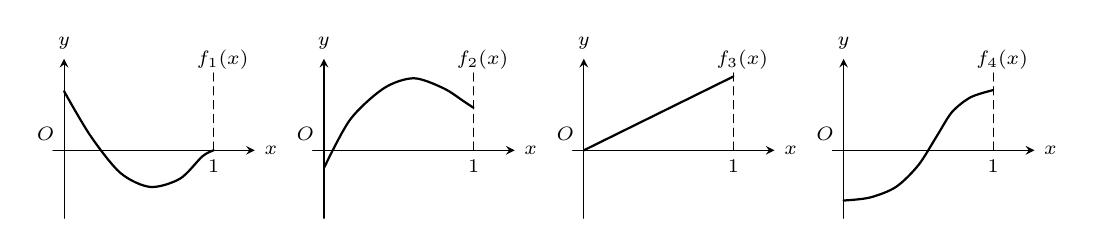
\begin{tikzpicture}[x=.95cm,y=.75cm,>=stealth,line cap=round,line join=round,
  every node/.style={font=\scriptsize}]
\foreach \shift/\name in {0/{f_1(x)},3.3/{f_2(x)},6.6/{f_3(x)},9.9/{f_4(x)}} {
  \begin{scope}[xshift=\shift cm]
    \draw[->] (-.15,0)--(2.55,0) node[right] {$x$};
    \draw[->] (0,-1.15)--(0,1.55) node[above] {$y$};
    \node[above left] at (0,0) {$O$};
    \node[above] at (2.12,1.2) {$\name$};
    \draw[densely dashed] (2,0)--(2,1.32);
    \node[below] at (2,0) {$1$};
  \end{scope}
}
% f_1: bowl-like (convex) curve.
\begin{scope}
  \draw[thick] plot[smooth] coordinates {(0,1.0) (.35,.25) (.75,-.38) (1.15,-.62) (1.55,-.48) (1.85,-.10) (2,0)};
\end{scope}
% f_2: arch-like (concave) curve; the endpoint at x=1 is part of [0,1].
\begin{scope}[xshift=3.3cm]
  \draw[thick] plot[smooth] coordinates {(0,-.3) (.35,.52) (.8,1.05) (1.2,1.22) (1.6,1.05) (1.88,.82) (2,.72)};
\end{scope}
% f_3: increasing line segment from the origin to the right endpoint.
\begin{scope}[xshift=6.6cm]
  \draw[thick] (0,0)--(2,1.25);
\end{scope}
% f_4: S-shaped curve with a change of concavity, qualitative only.
\begin{scope}[xshift=9.9cm]
  \draw[thick] plot[smooth] coordinates {(0,-.85) (.35,-.8) (.7,-.62) (1,-.25) (1.25,.25) (1.45,.65) (1.7,.9) (2,1.02)};
\end{scope}
\end{tikzpicture}
